\documentclass[11pt,a4paper]{article} % ein Artikel in 11-Punkt Schrift
% wie man sich schon denkt leitet % einen Kommentar bis Zeilenende ein

\usepackage[german]{babel} % deutsche Rechtschreibung
\usepackage[utf8]{inputenc} % Unicode Text 
\usepackage[T1]{fontenc} % Umlaute und deutsches Trennen
\usepackage{mathptmx} % Times New Roman, gewohnter Font
\usepackage{courier} % Schreibmaschinenfont schicker
\usepackage[scaled=.95]{helvet} % was serifenloses wenn gebraucht
\usepackage{graphicx} % wir wollen Bilder einfügen

\usepackage{listings} % Schöne Quellcode-Listings
\lstset{basicstyle=\sffamily, columns=[l]flexible, mathescape=true, 
  showstringspaces=false, numbers=left, numberstyle=\tiny}
\lstset{language=python} % und nur schöne Programmiersprachen ;-)
% und eine eigene Umgebung für Listings
\usepackage{float}
\newfloat{listing}{htbp}{scl}[section]
\floatname{listing}{Listing}

% Auch wenn es anrüchig ist, man kann den Platz etwas mehr ausnützen
\usepackage[paper=a4paper,width=14cm,left=35mm,height=22cm]{geometry}
\usepackage{setspace}
\linespread{1.15} % nicht ganz anderthalbzeilig, nur ein bisschen mehr Platz
\setlength{\parskip}{0.2em} % kleiner Paragraphenabstand
\setlength{\parindent}{0em} % im Deutschen Einrückung nicht üblich, leider

% Seitenmarkierungen 
\newcommand{\phv}{\fontfamily{phv}\fontseries{m}\fontsize{9}{11}\selectfont}
\usepackage{fancyhdr} % Schickere Header und Footer
\pagestyle{fancy}
% \addtolength{\headheight}{1ex} 
\fancyhead[L]{Ausarbeitung}
\fancyhead[R]{\thepage}
\fancyfoot[L]{Hochschule RheinMain}
\fancyfoot[C]{\ } % keine Seitenzahl unten
\fancyfoot[R]{Medieninformatik}

% Ein spezielles Paket zum Aufteilen des Literaturverzeichnisses
\usepackage{bibtopic}

\usepackage{blindtext} % damit wir nicht so viel tippen müssen, nur für Demo

\title{Ausarbeitung in \LaTeX}
\author{Medieninformatik}
\date{An einem Donnerstagmorgen \ldots } % oder \today für heute

\begin{document}
\maketitle % erzeugt den Titel mit Autor und Datum

\begin{abstract}
Im \emph{abstract} steht die Zusammenfassung.
\LaTeX\ wird an einem einfachen Beispiel vorgestellt. 
Das Beispiel sollte schon alles Notwendige enthalten, 
was man für eine Seminararbeit braucht. 
Es wird die Dokumentenstruktur aus Verzeichnissen, Abschnitten
und Paragraphen verdeutlicht. 
Wie man Bilder, Tabellen oder Listings einbringt wird gezeigt und 
auch der Formelsatz wird an einem Beispiel erläutert. 
Selbst Quellen und deren klare Trennung in Literatur und Online-Quellen
wird demonstriert.
\end{abstract}

\tableofcontents % das Inhaltsverzeichnis
\newpage % neue Seite, muss bei einem Artikel eigentlich nicht sein

\section{Einführung} \label{sec:einf} 
% mit \label können wir die Einführung referenzieren

Man kann in \LaTeX\ einfach % das \ am Ende von Kommandos, 
                            % damit da auch ein Leerzeichen kommt
seinen Quelltext schreiben und dann darauf vertrauen, dass es ordentlich 
(um)gesetzt wird. 
Zusätzlich verwendet man \emph{Markup}, der mit einem 
\verb|\|~(Backslash) eingeleitet wird.
Wie man sieht werden bei \LaTeX\ die Zeilenumbrüche ignoriert.

Ein neuer Absatz fängt an, wenn man im Quelltext eine Leerzeile schreibt.
Es ist eine gute Konvention Sätze immer in einer eigenen Zeile beginnen zu lassen.
In einem Text kann ein Teil des Textes \emph{hervorgehoben} werden.
Dies wird von \LaTeX meistens mit \textit{italic} umgesetzt. 
Man vermeidet \textbf{Fettschrift} im Fließtext.

\textit{
Es kann jedoch auch zum Beispiel ein ganzer Absatz \textit{italic} gesetzt
werden. 
Eine \emph{Hervorhebung} funktioniert dann immer noch.
}

Das \LaTeX\-System basiert auf dem 
\TeX\-System~\cite{knuth} % mit \cite wird zitiert
% Verwenden Sie bibtex als Literaturdatenbank
% Bibtex-Dateien sind einfach Text-Dateien mit .bib Endung
% mit Einträgen in einem speziellen Format. 
% Siehe ausarb.bib
von Donald E.~Knuth % ~ ist das nonbreaking space
und bietet viele nette Features.
Man kann Aufzählungen machen,
\begin{itemize}
\item Eins
\item Zwei
\item Drei
\end{itemize}
wenn man will auch nummerierte
\begin{enumerate}
\item Eins
\item Zwei
\item noch mehr
\begin{itemize}
\item Eins
\item Zwei
\item noch mehr
\end{itemize}
\end{enumerate}
und all das kann beliebig verschachtelt sein.
Um etwas Text zu produzieren verwenden wir das Paket
\textsf{blindtext}.

\Blindtext[1] % Das erzeugt einen Absatz

\subsection{Motivation}
\Blindtext[2] % Das erzeugt zwei Absätze

\subsection{Ziel}
\Blindtext[2] % Das erzeugt zwei Absätze

\subsection{Struktur}
\Blindtext[2] % Das erzeugt zwei Absätze


\section{Mittelteil} \label{sec:mittelteil}

Wir haben schon am Anfang der Einführung im Abschnitt~\ref{sec:einf} 
auf Seite~\pageref{sec:einf} ein \verb|\label| verwendet mit dem wir
(je nach Struktur) passend andere Textteile referenzieren können.
Das geht natürlich auch mit Mathematik -- gerade Mathematik geht 
besonders gut in \LaTeX.
\begin{equation} \label{eq:gauss}
  \sum_{i=1}^n i = \frac{n \cdot (n+1)}{2}
\end{equation}
Die Gleichung $\sum_{i=1}^n i = \frac{n \cdot (n+1)}{2}$ wird
im Fließtext passend gesetzt, also anders als 
Gleichung~(\ref{eq:gauss}). 
Man kann natürlich auch Code-Listings angeben -- zum Beispiel in Python.
\lstset{language=python}
\begin{lstlisting}
def ggt(x, y):
    while x != 0:
       x,y = y%x, x
    return y
\end{lstlisting}
Wenn man die Parameter für ein Listing einmal gesetzt hat, dann kann
man es immer wieder so verwenden. 
Wir müssen die Sprache also nicht noch einmal setzen, probieren 
aber mal schönere Fonts, Größen und Zeilennummern für Listings aus.
\lstset{basicstyle=\sffamily, columns=[l]flexible, mathescape=true, showstringspaces=false, numbers=left, numberstyle=\tiny}
\begin{lstlisting}
def ggt(x, y):
    while x != 0:
       x,y = y%x, x
    return y
\end{lstlisting}
Im Fließtext müssen Sonderzeichen gequotet werden wie z.B. \~{} , etc. 
Sonderzeichen werden meist mit $\backslash$ gequotet.

\section{Schluss} \label{sec:schluss}

Tabellen setzen und Bilder hinzufügen ist kein Problem. 
Tabellen und Bilder sollten als Fließobjekte (\emph{floats}) gesetzt werden.
Das heißt \LaTeX\ entscheidet wohin das Objekt kommt, man selbst
gibt nur Hinweise wo es gut wäre.

\begin{table}[htbp] % htbp ~ here, top, bottom, page
\centering
\begin{tabular}{|r|c|l|}
\hline
\textbf{Name} & \textbf{Wohnort} & \textbf{Telefon} \\ 
\hline
Susi Sinnlos & Eichenstrasse & 249274928749242 \\
hkurz & bla & 42 \\\hline
\end{tabular}
\caption{Adressliste}
\label{tab:meinetab}
\end{table}

Neben einer Tabelle wie in Tabelle~\ref{tab:meinetab} kann man 
auch eine Zeichnung als Fließobjekt nehmen.
Als Quelle nimmt man dafür am besten 
EPS (Encapulated Postscript\cite{postscript}) wenn
man mit \LaTeX\ arbeitet.
Alternativ kann man auch PDF-\LaTeX\ nehmen und
hat dann die Möglichkeit direkt PDF, JPG und PNG einzubinden.

\begin{figure}[htp]
\centering
% 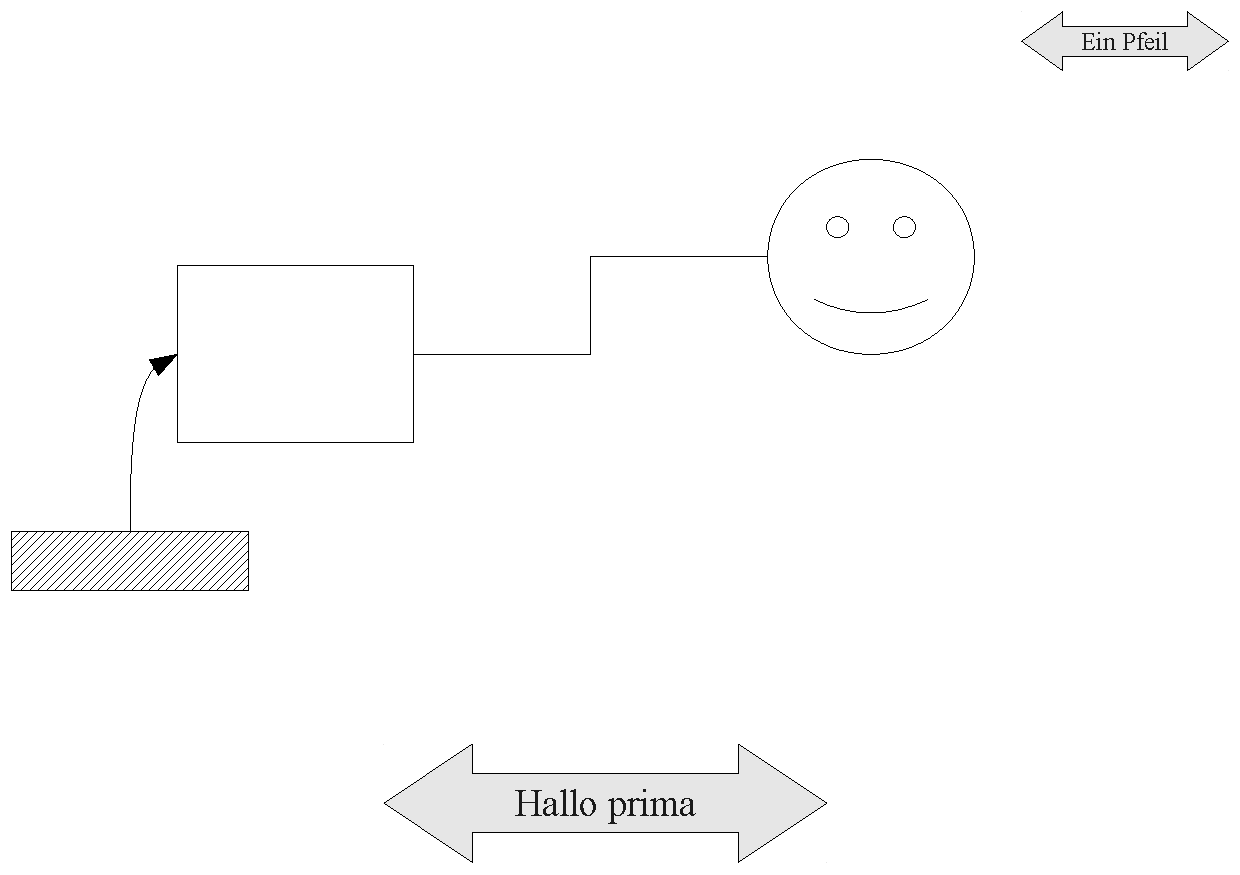
\includegraphics[width=.9\textwidth]{zeichnung.eps}
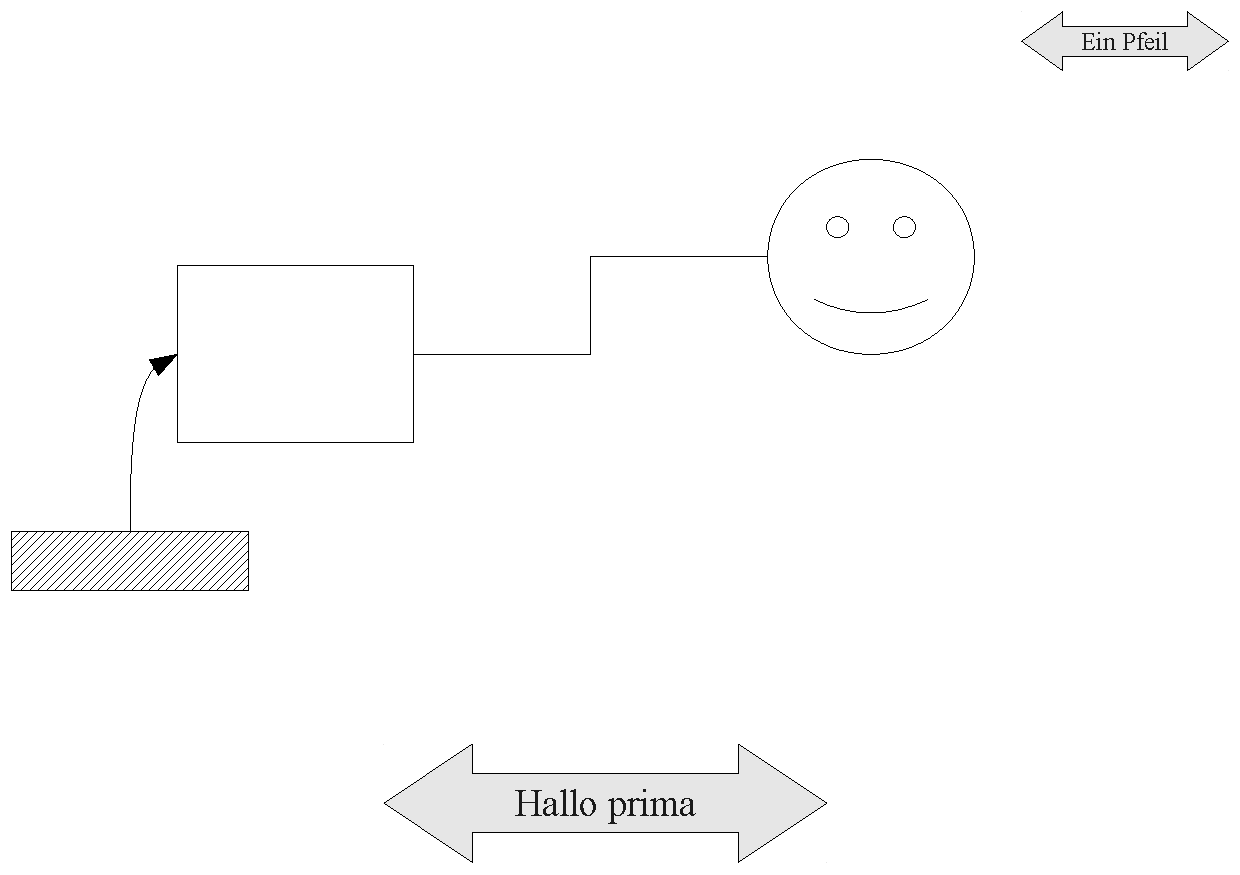
\includegraphics[width=.9\textwidth]{zeichnung.pdf}
\caption{Die tolle Konzeptzeichnung}
\label{fig:tk}
\end{figure}

Auch wenn der Code mal länger wird, wie in Abbildung~\ref{code:ggtaua}, 
was ja eigentlich in einer Ausarbeitung gar nicht vorkommt, 
dann sollte man den Code als Fließobjekt setzen und 
zusätzlich auch nie so lange Text schreiben wie der hier, der sich 
über mehre Zeilen zieht und einen ganzen Absatz repräsentiert, 
weil viele lange Text einfach nicht lesbar finden und man schnell
die Übersicht verliert, was hier passiert ist.
Kurze Sätze sind besser. 

\begin{listing}[ht]
\begin{lstlisting}
def ggt(x, y):
	if x == y or x == 1 or y == 1:
		return min(x,y)
	if x > y:
		x,y = y,x
	# es gilt x < y
	return ggt(x, y-x)
\end{lstlisting}
\caption{Listing ggt -- lang und schlecht}
\label{code:ggtaua}
\end{listing}

\Blindtext[2]

Und wenn man dann am Schluss ein PDF~\cite{pdf} macht, dann
sollten darin auch die Fonts gut aussehen. 
Die Fonts sollen beim Vergrößern nicht pixeln (Bitmap-Fonts) sondern
schön skalieren. 
Dazu war am Anfang die Zeile 
\begin{verbatim}
  \usepackage{cmlgc}
\end{verbatim}
oder die Zeile
\begin{verbatim}
  \usepackage{mathptmx}
\end{verbatim}
da.
Letztere verwendet Postscript-Times Schriften statt Computer Modern Roman
und das sieht auf günstigen Druckern ($< 2400$ dpi) besser aus.
Jetzt nochmal eine sinnlose Online-Quelle~\cite{wikipediaciting}.

\section{Zusammenfassung und Ausblick}

\LaTeX\ ist also cool und kann noch viele andere Dinge wie Farbe,
malen\footnote{In \LaTeX\ zu malen ist nur was für Hartgesottene.},
rechnen \ldots -- aber dazu gibt es ausreichend Doku, 
wie zum Beispiel den Kopka~\cite{kopka}.



\newpage

% Listen bitte ans Ende und nicht an den Anfang
\listoffigures % Liste der Abbildungen 
\listoftables % Liste der Tabellen

\newpage

% Als letztes noch das Literaturverzeichnis
\bibliographystyle{plain}
% so wäre es ganz einfach!
%\bibliography{ausarb,online}
% dann mit "bibtex ausarb" bibtexen und das Literaturverzeichnis ist da

% z.B. mit bibtopic kann man die Quellen sauber trennen
\begin{btSect}{ausarb}
\section*{Literaturverzeichnis}
\btPrintCited
\end{btSect}
\begin{btSect}{online}
\section*{Online-Quellen}
\btPrintCited
\end{btSect}
% dann mit "bibtex ausarb1" und "bibtex ausarb2" arbeiten

\end{document}
